\subsection{Analysis} \label{subsec:KListAnalysisL2}

In this section we analyze the complexity of Alg.~\ref{alg:AlgConfig} for the Configuration problem. First, we should mention that the memory complexity is completely determined by the input list-sizes $\abs{L_i}$ (remember that we restrict to constant $k$) and the application of $k$ filters does not change the asymtotics. In practice, all intermediate lists $L_i^{(j)}$ can be implemented by storing pointers to the elements of the original lists. 

In the following, we compute the expected sizes of filtered lists $L_i^{(j)}$ and establish the expected running time of Alg.~\ref{alg:AlgConfig}. Since our algorithm has an exponential running time $2^{cn}$ for some $c = \Theta(1)$, we are interested in determining $c$. We ignore polynomial factors, e.g.\ we do not take into account time spent for computing inner products. 

\begin{thm}\label{thm:RunTimeAlg1}
Let $k$ be fixed. Alg.~\ref{alg:AlgConfig} given as input $k$ lists $L_1, \ldots, L_k \subset \Sphere{n}$ of the same size $\abs{L}$, a target balanced configuration $\Cbalt \in \R^{k \times k}$, a target length $0 < t < \sqrt{k}$, and $\eps > 0$, outputs the list $\Lout$ of solutions to the Configuration problem. The expected running time of Alg.~\ref{alg:AlgConfig} is
	\begin{equation}\label{eq:RunTime}
	 T =  \softO \Bigl( \abs{L} \cdot \max\limits_{1 \leq i \leq k-1}  \abs{L}^i \cdot \frac{(k^2-t^2)^i}{(k^2-k)^{i+1}}  \cdot \Bigl( \frac{(k^2 - k + (i-1)(t^2-k))^2}{k^2 - k +(i-2)(t^2-k)} \Bigr)^{\frac{n}{2}} \Bigr).
  \end{equation}
In particular, for $t=1$ and $\abs{\Lout} = \abs{L}$ it holds that
  \begin{equation}\label{eq:RunTime=1}
	 T = \softO \biggl( \Bigl( \frac{k^{ \frac{1}{k-1} }}{k+1} \cdot  \max\limits_{1 \leq i \leq k-1} k^{\frac{i}{k-1}} \cdot \frac{(k-i+1)^2}{k-i+2}  \Bigr)^{\frac{n}{2}} \biggr).
  \end{equation}
\end{thm}

\begin{remark}\label{rmk:RunningTimeOfBLS} In the proof below we also show that the expected running time of 
the BLS
$k$-List algorithm 
from \cite{BLS16} for $t=1,\abs{\Lout}=\abs{L}$ is
\begin{equation} \label{eq:RunTimeBLS}
	T_{\text{BLS}} = \softO \Bigl(  \Bigl( \frac{k^{\frac{k}{k-1}}}{(k+1)^2} \cdot \max\limits_{1 \leq i \leq k-1} \bigl( k^{\frac{i}{k-1}} \cdot (k-i+1) \bigr)\Bigr)^{\frac{n}{2}} \Bigr).
\end{equation}
\end{remark} 

\begin{proof}[Proof of Thm.~\ref{thm:RunTimeAlg1}]
	The correctness of the algorithm is straightforward: let us associate the lists $L^{(i)}$ with a level $i$, where $i$ indicates the number of filtering steps applied to $L$ (we identify the input lists with the $0\th$ level: $L_i=L^{(0)}_i$). So for executing the filtering for the $i\th$ time, we choose an $\xvec_{i} \in L_{i}^{(i-1)}$ that satisfies the condition $\abs{\ScProd{\xvec_i}{\xvec_{i-1}} - C_{i,i-1}} \leq \eps$ (for a fixed $\xvec_{i-1}$) and append to a previously obtained $(i-1)$-tuple $(\xvec_1, \ldots, \xvec_{i-1})$. Thus, on the last level, we put into $\Lout$ a $k$-tuple $(\xvec_1, \ldots, \xvec_{k})$ that is a solution to the Configuration problem. To make the subscripts less confusing, we set $C = \Cbalt$ throughout the proof. 
	
	Let us first estimate the size of the list $L_i^{(i-1)}$ output by the filtering process applied to the list $L_i^{(i-2)}$ for $i>1$ (i.e.\ the left-most lists in Fig.~\ref{fig:AlgDescription}). Recall that all $\xvec_i \in L_i^{(i-1)}$ satisfy $\abs{\ScProd{\xvec_i}{\xvec_{j}} - C_{i,j}} \leq \eps$, $1 \leq j \leq i-1 $. Then the \emph{total} number of $i$-tuples $(\xvec_1, \xvec_2, \ldots, \xvec_i) \in L_1 \times L_2^{(1)} \times \ldots \times L_i^{(i-1)}$ considered by the algorithm is determined by the probability that in a random $i$-tuple, all pairs $(\xvec_j, \xvec_{j'}), 1 \leq j,j' \leq i$ satisfy the inner product constraints given by $C_{j,{j'}}$. This probability is given in Thm.~\ref{thm:WishartDist} and, since the input lists are of the same size $\abs{L}$, we have\footnote{Throughout this proof, the equations that involve list-sizes $\abs{L}$ and running time $T$ are assumed to have $\softO(\cdot)$ on the right-hand side. We omit it for clarity.}
	\begin{align}\label{eq:ProductOfListSizes}
			\normalabs{L_1} \cdot \normalabs{L_2^{(1)}} \cdot \ldots \normalabs{L_i^{(i-1)}} = \normalabs{L}^i \cdot  \det (C[1 \ldots i])^{\frac{n}{2}},
	\end{align}	
where $\det(C[1 \ldots i])$ denotes the $i$-th principal minor of $C$.
Using Eq.~\eqref{eq:ProductOfListSizes} for two consecutive values of $i$ and dividing one equation by the other, we obtain
	\begin{align}\label{eq:IntermSize}
		\normalabs{L_{i+1}^{(i)}} = \abs{L} \cdot \Bigl( \frac{\det (C[1 \ldots i+1]}{\det (C[1 \ldots i])} \Bigr)^{\frac{n}{2}}.
	\end{align}
Note that these expected list sizes can be smaller than 1. This should be thought of as the inverse probability that the list is not empty.
Since our target is a balanced configuration $\Cbalt$, the entries of the input Gram matrix are specified by Thm.~\ref{thm:maxConfig} and, hence, we compute the determinants in the above quotient by applying Lemma~\ref{lem:CBalancedDet} with $a = \frac{t^k-k}{k^2-k}$. Again, from the shape of the Gram matrix $\Cbalt$ and the equally-sized input lists, it follows that the filtered list on each level are of the same size: $\normalabs{L_{i+1}^{(i)}} = \normalabs{L_{i+2}^{(i)}} = \ldots = \normalabs{L_k^{(i)}}$. Therefore, for all filtering levels $0 \leq j \leq k-1$ and for all $j+1 \leq i \leq k$,
  \begin{equation}\label{eq:IntermSizeExpanded}
	 \bigabs{L_i^{(j)}} = \abs{L} \cdot \Bigl( \frac{k^2 - t^2}{k^2 - k} \cdot \frac{k^2 - k + j(t^2-k)}{k^2 - k +(j-1)(t^2-k)} \Bigr)^{ \frac{n}{2} }.
  \end{equation}
Now let us discuss the complexity of the algorithm. Clearly, the running time of Alg.~\ref{alg:AlgConfig} is (up to sub-exponential factors in $n$) 
\begin{align*}
   T = \normalabs{L_1^{(0)}} \cdot (\normalabs{L_2^{(0)}} + \normalabs{L_2^{(1)}} \cdot (\normalabs{L_3^{(1)}} +\normalabs{L_3^{(2)}} \cdot(\ldots \cdot (\normalabs{L_k^{(k-2)}} + \normalabs{L_k^{(k-1)}} ) )).
\end{align*}  
Multiplying out and observing that $\normalabs{L_k^{(k-2)}}>\normalabs{L_k^{(k-1)}}$ (so creating a filtered list takes longer than enumerating over it), we may ignore the very last term and deduce that the total running time is (up to sub-exponential factors) given by

  \begin{equation} \label{eq:RunTimeProof}
  	T =  \abs{L} \cdot \max\limits_{1 \leq i \leq k-1}  \normalabs{L^{(i-1)}} \cdot \prod_{j=1}^{i-1} \normalabs{L^{(j)}},
  \end{equation}
  where $\normalabs{L^{(j)}}$ is the size of any filtered list on level $j$ (so we omit the subscripts). Consider the value $\im$ of $i$, where the maximum is attained in the above formula. The meaning of $\im$ is that the total cost over all loops to create the lists $L_j^{(\im)}$ dominates the running time. At this level, the lists $L_j^{(\im)}$ become small enough such that iterating over them (i.e.\ creating $L_j^{(\im+1)}$) does not contribute to the asymptotics. Plugging in Eqns.~\eqref{eq:ProductOfListSizes} and \eqref{eq:IntermSize} into Eq.~\eqref{eq:RunTimeProof}, we obtain
  \vspace{-1ex}
  \begin{equation}\label{eq:TotalRunningTimeViaDets}
    T=\abs{L}\cdot \max\limits_{1\le i \leq k-1} \normalabs{L}^i \Bigl( \frac{(\det C[1\ldots i])^2}{\det C[1\ldots (i-1)]}\Bigr)^{\frac{n}{2}}.
  \end{equation}
  From Lemma~\ref{lem:CBalancedDet}, $\det C[1\ldots i] = \Bigl( 1 + (i-1)\frac{t^2-k}{k^2-k})\Bigr) \Bigl( \frac{k^2-t^2}{k^2-k} \Bigr)^{i-1}$, giving us the desired expression for the running time.
  
  For the case $t=1$ and $\normalabs{\Lout} = \normalabs{L}$, the result of Cor.~\ref{cor:BalancedListSizes} on the size of the input lists $\abs{L}$ yields a compact formula for the filtered lists:
    \vspace{-1ex}
    \begin{equation}\label{eq:IntermSize_t=1}
    	\bigabs{L_i^{(j)}} =  \Bigl( k^{\frac{1}{k-1}} \cdot \frac{k-j}{k-j+1} \Bigr)^{\tfrac{n}{2}}.
    \end{equation}
    Plugging this into either Eq.~\eqref{eq:RunTimeProof} or Eq.~\eqref{eq:TotalRunningTimeViaDets}, the running time stated in Eq.~\eqref{eq:RunTime=1} easily follows.
    
    It remains to show the complexity of the BLS algorithm \cite{BLS16}, claimed in Rmk.~\ref{rmk:RunningTimeOfBLS}. The algorithm is illustrated in Fig.~\ref{fig:AlgBLS}. We change the presentation of the algorithm to our configuration setting: in the original description, a vector $\xvec_i$ survives the filter if it satisfies $\abs{ \ScProd{\xvec_i}{\xvec_1 + \ldots + \xvec_{i-1}}} \geq c_i$ for a predefined $c_i$ (a sequence $(c_1, \ldots, c_{k-1}) \in \R^{k-1}$ is given as input to the BLS algorithm). Our concentration result (Thm.~\ref{thm:WishartDist}) also applies here and the condition $\abs{ \ScProd{\xvec_i}{\xvec_1 + \ldots + \xvec_{i-1}}} \geq c_i$ is equivalent to a pairwise constraint on the scalar product $\ScProd{\xvec_i}{\xvec_j}$ up to losing an exponentially small fraction of solutions. The optimal sequence of $c_i$'s corresponds to the configuration $\Cbalt$ derived in Thm.~\ref{thm:maxConfig}.
    
    Indeed, Table 1 in \cite{BLS16} matches $\Cbalt$ (case $t=1$) exactly. So we may rephrase their filtering where instead of shrinking the list $L_i$ by taking inner products with the sum $\xvec_1+ \ldots + \xvec_{i-1}$, we filter $L_i$ by considering $\ScProd{\xvec_i}{\xvec_j}$ for $1 \leq j \leq i-1$. 
      
    It follows that the filtered lists $L^{(i)}$ on level $i$ are of the same size (in leading order) for both our and BLS algorithms.
    In particular, Eq.~\eqref{eq:IntermSize} holds for the expected list-sizes of the BLS algorithm.
    
    The crucial difference lies in the construction of these lists. To construct the list $L_i^{(i-1)}$ in BLS, the filtering procedure is applied not to $L_i^{(i-2)}$ but to a (larger) input-list $L_i$. Hence, the running time of the BLS algorithm ignoring sub-exponential factors, is (cf.\ Eq.~\eqref{eq:RunTimeProof})
      \begin{align*}
      	 T_{BLS} = 
      	 \normalabs{L_1} \cdot (\normalabs{L_2} + \normalabs{L_2^{(1)}} \cdot ( \normalabs{L_3} +\normalabs{L_3^{(2)}}  \cdot(\ldots \cdot (\normalabs{L_k} + \normalabs{L_k^{(k-1)}} ) ))
    	 =
      	 \normalabs{L}^2 \cdot \max\limits_{1 \leq i \leq k-1} \cdot \prod_{j=1}^{i-1} \normalabs{L^{(j)}}.
      \end{align*}
    The result follows after substituting Eq.~\eqref{eq:IntermSize_t=1} into the above product. 
\end{proof}

Both runtime expressions, Eq.~\eqref{eq:RunTime} for Alg.~\ref{alg:AlgConfig} and Eq.~\eqref{eq:RunTimeBLS} for the BLS algorithm, can be easily evaluated given $k$ and $\normalabs{L}$, see Fig.~\ref{fig:RunTimes}. The input list-sizes $\normalabs{L}$ are chosen to guarantee $\normalabs{\Lout} = \normalabs{L}$ on expectation.

\begin{SCfigure}[1.2]
	\centering
	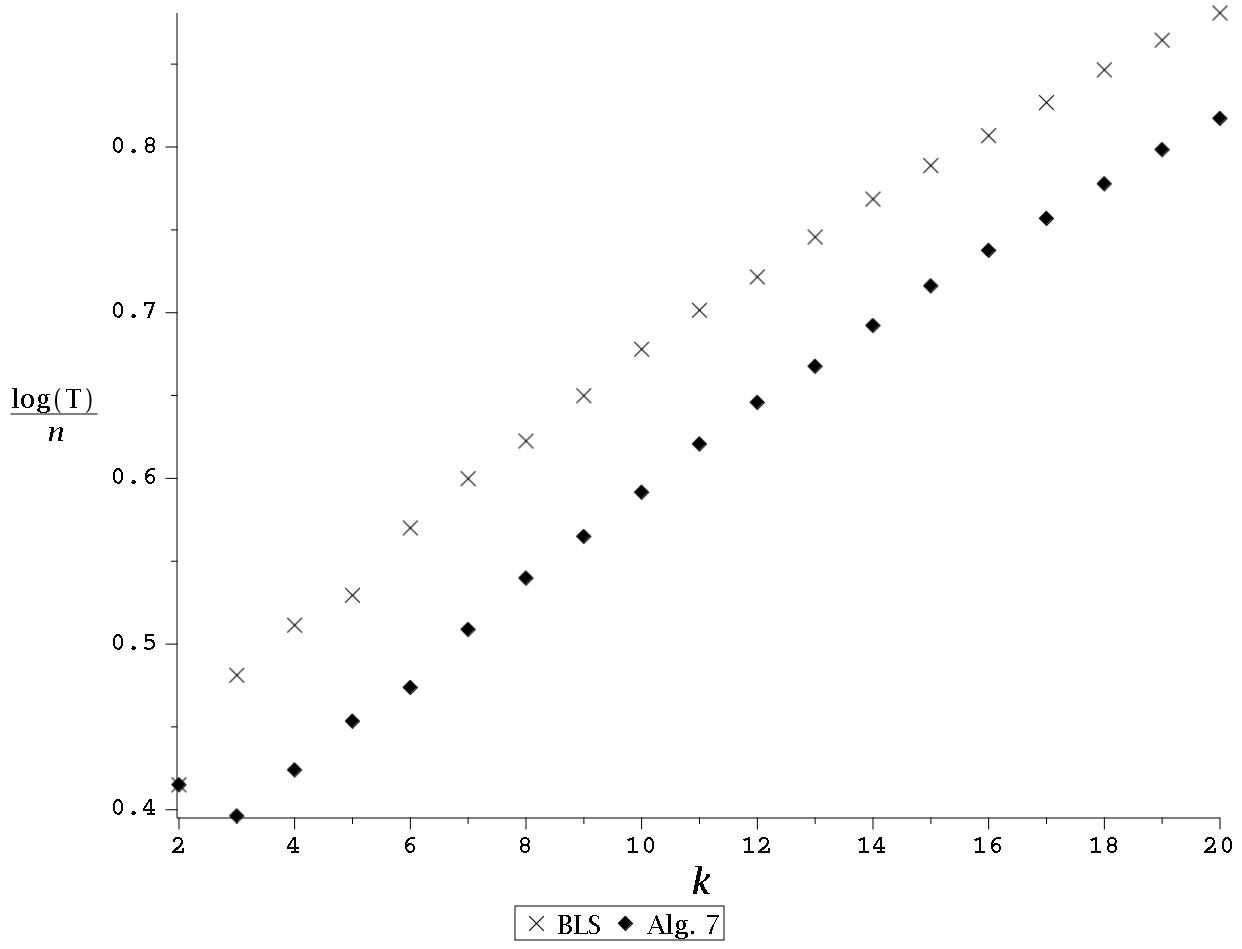
\includegraphics[scale=0.2]{kListRunTimesCompare}
	\hspace{4ex}
	\caption[Runtime exponents for $k$-List algorithms]{Running time exponents scaled by $1/n$ for the target length $t=1$. For $k=2$, both algorithms are the Nguyen-Vidick sieve \cite{NguVid08} with $\log(T)/n = 0.415$ (naive brute-force over two lists). For $k=3$, Algorithm \ref{alg:AlgConfig} achieves $\log(T)/n = 0.3962$, the BLS algorithm has $\log(T)/n = 0.4812$. \vspace{10ex}} \label{fig:RunTimes}
\end{SCfigure}

Our algorithm can be further improved by applying Locality-Sensitive Hashing techniques similar to \cite{SODA:BDGL16} to shorten the lists prior to filtering. Unfortunately, the gain is very modest: for $k=3, t=1$, we can get the running time down from $2^{0.3962n + \smallo(n)}$ to $2^{0.3717n + \smallo(n)}$. The details on this extension are presented in \cite{HK}.

We remark that it seems quite challenging to analyze the $k$-List algorithms for a \emph{non-fixed} $k$. Our approach heavily relies on the fact that $k$ is a fixed constant allowing to suppress all the pre-factors in both run-times and list sizes in the $\softO_k(\cdot)$ notation. Indeed, taking a closer look at the suppressed pre-factors, we immediately notice that they depend at least \emph{exponentially} on $k$ (see, for example, the expression for $W_{n,k}$ in Thm.~\ref{thm:WishartDist}). Being able to let $k \rightarrow \infty$ would, however, greatly contribute to our understanding of complexity of \SVP as it would enable us to compare sieving techniques with enumeration. 

Further, we do not know what is an optimal choice of $\eps$ given $k$ and $\normalabs{L}$. In Sect.~\ref{subsec:KListResults}, we present our experimental results for Alg.~\ref{alg:AlgConfig}, where we just try several $\eps$'s.